% =====================================================================
%  SheafCovPool graph readout  (Figure 5, single column)
%
%  Design rule (shared with h2snn_overview.tex): DRAW the object, do not
%  describe it in a text box.  Text appears only as (i) a short symbol
%  attached to a drawn object, (ii) an operator name on an arrow, or
%  (iii) an equation tag pointing back into the manuscript.
%
%  Colour semantics -- fixed across the whole figure:
%    cA  blue   : the diffused node state  x^*   and what it induces
%    cP  slate  : the initial typed state  h^(0) and what it induces
%    grn green  : the edge cochain         s^*   and what it induces
%    gold       : learned weights (attention a_i)
%    tealx      : gauge freedom / invariance
%    rose       : prediction head
%  Node branch = upper lane, edge branch = lower lane; lane identity is
%  carried by the wash tint and by subscripts (Z_v/Z_e, mu_0/mu_1).
%
%  Equation numbers are pulled live from ../h2snn_manuscript.aux via xr,
%  so they never go stale.  Compile from paper/figure/ :
%      latexmk -pdf sheafcovpool_architecture.tex
%  Natural width is 8.43cm ~ \columnwidth of acmart[sigconf], so the
%  figure is included at scale ~1 and labels keep their true size.
% =====================================================================
\documentclass[tikz,border=2pt]{standalone}
\usepackage{amsmath,amssymb}
\usepackage{libertine}
\usepackage[libertine]{newtxmath}
\usepackage{xr}
\externaldocument{../h2snn_manuscript}
\usetikzlibrary{arrows.meta,positioning,calc,backgrounds,decorations.pathreplacing}

% ---------- palette (Paul Tol, colour-blind safe) ----------
\definecolor{ink}  {HTML}{243447}
\definecolor{cA}   {HTML}{4477AA}   % x^*   (diffused node state)
\definecolor{cP}   {HTML}{8899AA}   % h^(0) (initial typed state)
\definecolor{grn}  {HTML}{228833}   % s^*   (edge cochain)
\definecolor{gold} {HTML}{CCAA33}   % learned attention weights
\definecolor{tealx}{HTML}{44AA99}   % gauge / invariance
\definecolor{rose} {HTML}{AA3377}   % head

\newcommand{\R}{\mathbb{R}}
\newcommand{\eqn}[1]{{\tiny\color{ink!45}(\ref{#1})}}
\newcommand{\T}{^{\mathsf{T}}}

\begin{document}
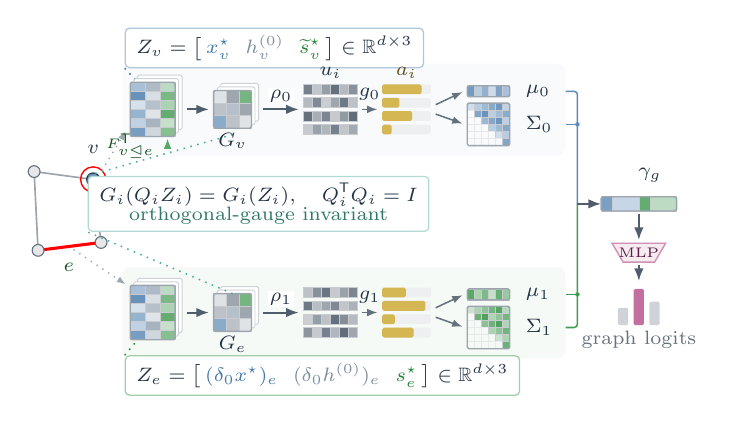
\begin{tikzpicture}[
  x=1cm,y=1cm,font=\scriptsize,text=ink,>=Latex,
  flow/.style  ={-{Latex[length=1.6mm]},line width=.7pt,draw=ink!80},
  thin flow/.style={-{Latex[length=1.3mm]},line width=.55pt,draw=ink!70},
  lead/.style  ={dotted,draw=ink!45,line width=.5pt,-{Latex[length=1.1mm]}},
  cell/.style  ={draw=ink!25,line width=.25pt},
  ghost/.style ={draw=ink!22,line width=.35pt,fill=white,rounded corners=.6pt},
  card/.style  ={draw=ink!45,line width=.5pt,rounded corners=.6pt},
  wash/.style  ={rounded corners=3pt,draw=none},
  lbl/.style   ={fill=white,inner sep=.7pt},
]

% ---------------- reusable drawing primitives ----------------
% one column of a view stack: x, ybase, colour, list "row/opacity"
\newcommand{\zcol}[4]{%
  \foreach \r/\o in {#4}{%
    \draw[cell,fill=#3!\o] (#1,{#2+0.115*\r}) rectangle ++(0.19,0.115);}}
% view stack Z in R^{d x 3}, drawn as a deck (one card per cell of the graph)
\newcommand{\zcard}[2]{%
  \draw[ghost] ({#1+0.09},{#2+0.09}) rectangle ++(0.57,0.69);
  \draw[ghost] ({#1+0.045},{#2+0.045}) rectangle ++(0.57,0.69);
  \fill[white] (#1,#2) rectangle ++(0.57,0.69);
  \zcol{#1}{#2}{cA}{0/72,1/34,2/56,3/22,4/80,5/46}
  \zcol{#1+0.19}{#2}{cP}{0/40,1/74,2/26,3/62,4/32,5/68}
  \zcol{#1+0.38}{#2}{grn}{0/54,1/26,2/70,3/38,4/60,5/30}
  \draw[card] (#1,#2) rectangle ++(0.57,0.69);}
% Gram descriptor G in R^{3x3}: diagonal = per-view energy, off-diagonal =
% cross-view alignment; symmetric opacities show G = G^T
\newcommand{\gcard}[2]{%
  \draw[ghost] ({#1+0.09},{#2+0.09}) rectangle ++(0.48,0.48);
  \draw[ghost] ({#1+0.045},{#2+0.045}) rectangle ++(0.48,0.48);
  \fill[white] (#1,#2) rectangle ++(0.48,0.48);
  \foreach \i/\j/\c in {0/0/{cA!62},1/1/{cP!62},2/2/{grn!62},
                        0/1/{ink!30},1/0/{ink!30},
                        0/2/{ink!14},2/0/{ink!14},
                        1/2/{ink!44},2/1/{ink!44}}{%
    \draw[cell,fill=\c] ({#1+0.16*\i},{#2+0.16*\j}) rectangle ++(0.16,0.16);}
  \draw[card] (#1,#2) rectangle ++(0.48,0.48);}
% token u_i in R^F : x, ybase, list "col/opacity"
\newcommand{\tokrow}[3]{%
  \foreach \c/\o in {#3}{%
    \draw[cell,fill=ink!\o] ({#1+0.115*\c},#2) rectangle ++(0.115,0.125);}}
% attention weight: x, ybase, filled length (track is the full unit)
\newcommand{\attn}[3]{%
  \fill[ink!8,rounded corners=.6pt] (#1,#2) rectangle ++(0.62,0.125);
  \fill[gold!85,rounded corners=.6pt] (#1,#2) rectangle ++(#3,0.125);}
% weighted mean mu_r in R^F
\newcommand{\murow}[3]{%
  \foreach \c/\o in {0/74,1/38,2/58,3/26,4/68,5/46}{%
    \draw[cell,fill=#3!\o] ({#1+0.09*\c},#2) rectangle ++(0.09,0.14);}
  \draw[card] (#1,#2) rectangle ++(0.54,0.14);}
% weighted covariance Sigma_r: only the upper triangle is kept by triu()
\newcommand{\covcard}[3]{%
  \foreach \i in {0,...,5}{\foreach \j in {0,...,5}{%
    \pgfmathtruncatemacro{\op}{24+mod(13*\i+29*\j,56)}
    \ifnum\i<\j
      \draw[draw=ink!11,line width=.2pt]
        ({#1+0.09*\i},{#2+0.54-0.09*(\j+1)}) rectangle ++(0.09,0.09);
    \else
      \draw[cell,fill=#3!\op]
        ({#1+0.09*\i},{#2+0.54-0.09*(\j+1)}) rectangle ++(0.09,0.09);
    \fi}}
  \draw[card] (#1,#2) rectangle ++(0.54,0.54);}
% =====================================================================
%  LANE WASHES
% =====================================================================
\fill[wash,fill=cA!4]  (1.42,3.26) rectangle (7.05,4.42);
\fill[wash,fill=grn!4] (1.42,0.68) rectangle (7.05,1.84);

% =====================================================================
%  SOURCE GRAPH -- highlighted node v and edge e feed the two readout lanes
% =====================================================================
\coordinate (g1) at (0.30,3.05);
\coordinate (g2) at (1.05,2.95);
\coordinate (g3) at (1.15,2.15);
\coordinate (g4) at (0.35,2.05);
\foreach \s/\t in {g1/g2,g2/g3,g4/g1}
  {\draw[ink!45,line width=.6pt] (\s)--(\t);}
\draw[red,line width=1.1pt] (g3)--(g4);
\foreach \p in {g1,g3,g4}{\filldraw[fill=ink!12,draw=ink!70,line width=.4pt] (\p) circle (.075);}
\draw[red,line width=.5pt] (g2) circle (.16);
\filldraw[fill=cA!75,draw=ink,line width=.45pt] (g2) circle (.082);
\node[font=\scriptsize,anchor=south] at (1.05,3.16) {$v$};
\node[font=\scriptsize,text=grn!60!black,anchor=north] at (0.74,2.01) {$e$};
%\node[font=\scriptsize,text=ink!70] at (0.72,1.68) {graph $g$};

\draw[lead] (1.16,3.06) --  (1.46,3.56);
\draw[lead] (0.80,2.06) --  (1.46,1.62);

% =====================================================================
%  NODE LANE  (upper) -- centre y = 3.84
% =====================================================================
\node[
  anchor=west,
  draw=cA!42,
  fill=white,
  rounded corners=1.5pt,
  line width=.45pt,
  inner xsep=4pt,
  inner ysep=2.5pt,
  font=\scriptsize
] (zv-definition) at (1.45,4.62)
  {$Z_v=\bigl[\,
    \textcolor{cA}{x_v^\star}\ \
    \textcolor{cP!88!ink}{h_v^{(0)}}\ \
    \textcolor{grn}{\widetilde s_v^\star}
    \,\bigr]\in\R^{d\times3}$};

\draw[
  dotted,
  draw=cA,
  line width=.55pt
] (zv-definition.south west) -- (1.62,4.18);

\zcard{1.52}{3.495}
% The third node view is not a raw edge state: each incident s_e^* is pulled back
% through its own endpoint restriction map, so all three columns share one stalk.
\draw[thin flow,draw=grn!75] (1.995,3.34) -- (1.995,3.47);
\node[font=\tiny,text=grn!60!black,anchor=east] at (1.95,3.37) {$F_{v\unlhd e}\T$};
\draw[flow] (2.24,3.84) -- (2.52,3.84);
\gcard{2.58}{3.60}
\node[font=\scriptsize] at (2.82,3.44) {$G_v$};

\draw[flow] (3.21,3.84) -- (3.66,3.84);
\node[lbl,font=\scriptsize] at (3.435,4.01) {$\rho_0$};

\tokrow{3.72}{4.0325}{0/62,1/28,2/48,3/70,4/34,5/54}
\tokrow{3.72}{3.8625}{0/34,1/58,2/24,3/44,4/66,5/30}
\tokrow{3.72}{3.6925}{0/70,1/40,2/60,3/26,4/50,5/72}
\tokrow{3.72}{3.5225}{0/26,1/46,2/36,3/62,4/28,5/42}
\node[font=\scriptsize] at (4.065,4.30) {$u_i$};

\draw[thin flow] (4.46,3.84) -- (4.66,3.84);
\node[font=\scriptsize] at (4.56,4.03) {$g_0$};
\attn{4.72}{4.0325}{0.50}
\attn{4.72}{3.8625}{0.22}
\attn{4.72}{3.6925}{0.38}
\attn{4.72}{3.5225}{0.12}
\node[font=\scriptsize,text=gold!45!black] at (5.03,4.30) {$a_i$};

\draw[thin flow] (5.40,3.90) -- (5.74,4.06);
\draw[thin flow] (5.40,3.78) -- (5.74,3.66);
\murow{5.80}{4.00}{cA}
\covcard{5.80}{3.38}{cA}
\node[anchor=west,font=\scriptsize] at (6.42,4.07) {$\mu_0$};
\node[anchor=west,font=\scriptsize] at (6.42,3.65) {$\Sigma_0$};

% =====================================================================
%  EDGE LANE  (lower) -- centre y = 1.26
% =====================================================================
\zcard{1.52}{0.915}
\draw[flow] (2.24,1.26) -- (2.52,1.26);
\gcard{2.58}{1.02}
\node[font=\scriptsize] at (2.82,0.86) {$G_e$};

\draw[flow] (3.21,1.26) -- (3.66,1.26);
\node[lbl,font=\scriptsize] at (3.435,1.43) {$\rho_1$};

\tokrow{3.72}{1.4525}{0/30,1/54,2/68,3/26,4/46,5/60}
\tokrow{3.72}{1.2825}{0/66,1/32,2/44,3/58,4/28,5/38}
\tokrow{3.72}{1.1125}{0/24,1/48,2/30,3/70,4/56,5/34}
\tokrow{3.72}{0.9425}{0/52,1/26,2/62,3/36,4/72,5/44}

\draw[thin flow] (4.46,1.26) -- (4.66,1.26);
\node[font=\scriptsize] at (4.56,1.45) {$g_1$};
\attn{4.72}{1.4525}{0.30}
\attn{4.72}{1.2825}{0.55}
\attn{4.72}{1.1125}{0.16}
\attn{4.72}{0.9425}{0.40}

\draw[thin flow] (5.40,1.32) -- (5.74,1.48);
\draw[thin flow] (5.40,1.20) -- (5.74,1.08);
\murow{5.80}{1.42}{grn}
\covcard{5.80}{0.80}{grn}
\node[anchor=west,font=\scriptsize] at (6.42,1.49) {$\mu_1$};
\node[anchor=west,font=\scriptsize] at (6.42,1.07) {$\Sigma_1$};

\node[
  anchor=west,
  draw=grn!42,
  fill=white,
  rounded corners=1.5pt,
  line width=.45pt,
  inner xsep=4pt,
  inner ysep=2.5pt,
  font=\scriptsize
] (ze-definition) at (1.45,0.46)
  {$Z_e=\bigl[\,
    \textcolor{cA}{(\delta_0x^\star)_e}\ \
    \textcolor{cP!88!ink}{(\delta_0h^{(0)})_e}\ \
    \textcolor{grn}{s_e^\star}
    \,\bigr]\in\R^{d\times3}$};

\draw[
  dotted,
  draw=grn,
  line width=.55pt
] (ze-definition.north west) -- (1.62,0.92);

% =====================================================================
%  MIDDLE BAND -- the two properties the drawing cannot show by itself
% =====================================================================
\node[
  draw=tealx!42,
  fill=white,
  rounded corners=1.5pt,
  line width=.45pt,
  inner xsep=4pt,
  inner ysep=2.5pt,
  align=center,
  font=\scriptsize
] (gram-invariance) at (3.15,2.64)
  {$G_i(Q_iZ_i)=G_i(Z_i),\quad Q_i\T Q_i=I$\\[-1pt]
   \textcolor{tealx!70!black}{orthogonal-gauge invariant}};

% Connect the identity to the node- and edge-level Gram descriptors.
\draw[
  dotted,
  draw=tealx,
  line width=.55pt
] (2.82,3.52) -- (gram-invariance.north west);

\draw[
  dotted,
  draw=tealx,
  line width=.55pt
] (2.82,1.50) -- (gram-invariance.south west);
%\node[font=\scriptsize,text=tealx!68!black] at (3.05,2.42)
%  {for any stalk gauge $Q_i\in O(d)$};
%\node[font=\scriptsize,text=ink!70] at (5.90,2.42)
%  {$\textstyle\sum_{i\in\mathcal{C}_r(g)}a_i=1$};

% ---- four summaries ride one riser at x = 7.20, then ONE arrow enters the
%      bar: the merge itself is the picture of "concatenate".
\draw[rounded corners=1.2pt,line width=.55pt,draw=cA!85]
  (7.05,4.07) -- (7.20,4.07) -- (7.20,2.64);
\draw[line width=.55pt,draw=cA!85]  (7.05,3.65) -- (7.20,3.65);
\draw[rounded corners=1.2pt,line width=.55pt,draw=grn!85]
  (7.05,1.07) -- (7.20,1.07) -- (7.20,2.64);
\draw[line width=.55pt,draw=grn!85] (7.05,1.49) -- (7.20,1.49);
\fill[cA!85]  (7.20,3.65) circle (.028);
\fill[grn!85] (7.20,1.49) circle (.028);
\draw[flow] (7.20,2.64) -- (7.50,2.64);

\foreach \x/\w/\c in {7.50/0.14/{cA!70},7.64/0.34/{cA!30},
                      7.98/0.14/{grn!70},8.12/0.34/{grn!30}}{%
  \draw[cell,fill=\c] (\x,2.55) rectangle ++(\w,0.18);}
\draw[card] (7.50,2.55) rectangle ++(0.96,0.18);
\node[font=\scriptsize,anchor=south] at (8.12,2.79)
  {$\gamma_g$};

\draw[flow] (7.98,2.51) -- (7.98,2.18);
\draw[fill=rose!10,draw=rose!55,line width=.5pt]
  (7.64,2.14) -- (8.32,2.14) -- (8.18,1.90) -- (7.78,1.90) -- cycle;
\node[font=\tiny,text=rose!55!black] at (7.98,2.02) {MLP};
\draw[flow] (7.98,1.86) -- (7.98,1.66);
\fill[ink!22,rounded corners=.5pt] (7.715,1.10) rectangle ++(0.13,0.22);
\fill[rose!70,rounded corners=.5pt] (7.915,1.10) rectangle ++(0.13,0.46);
\fill[ink!22,rounded corners=.5pt] (8.115,1.10) rectangle ++(0.13,0.30);
\node[font=\scriptsize,text=ink!70] at (7.98,0.92) {graph logits};


\end{tikzpicture}
\end{document}
